\documentclass[10pt]{beamer}
\usetheme{Warsaw}
\usepackage[utf8]{inputenc}
\usepackage[english]{babel}
\usepackage{amsmath}
\usepackage{amsfonts}
\usepackage{amssymb}
\usepackage{wrapfig}
\usepackage{graphicx}
\usepackage{array}
\author{
\footnotesize
\textbf{
\linebreak Achyuth Rao - B120314254
\linebreak Akib Shaikh - B120314257
\linebreak Arun Pottekat - B120314203
\linebreak Pranav Tale - B120314249
\linebreak 
\linebreak
Guide:- Prof. Mrs. Aparna Junnarkar
}
}

\title{
\small
\textbf{
Detection of DDoS in SDN environment using Support Vector Machine, Entropy based discretization and Fuzzy C-Means Clustering
}
}
\date{}
\institute{

\includegraphics[width=2.3cm, height=2.9cm]{logo.png}\\ \textbf{PES's Modern College Of Engineering}} 
\setbeamertemplate{footline}[frame number]{}
\setbeamertemplate{navigation symbols}{} 
\setbeamertemplate{caption}[numbered]
\setbeamertemplate{section in toc}[ball unnumbered]
\begin{document}

\begin{frame}
\titlepage
\end{frame}


\begin{frame}
\frametitle{Contents}
\footnotesize
\tableofcontents
\end{frame}

\begin{frame}

\frametitle{Introduction}
\section[]{Introduction}
\begin{itemize}
\footnotesize
\item
SDN separates intelligence from the hardware.
\item
SDN controller acts as Network Operating System.
\item
This networking paradigm faces security issues.
%\item
\item
DDoS attack makes the network resources unavailable.
\end{itemize}
\begin{figure}
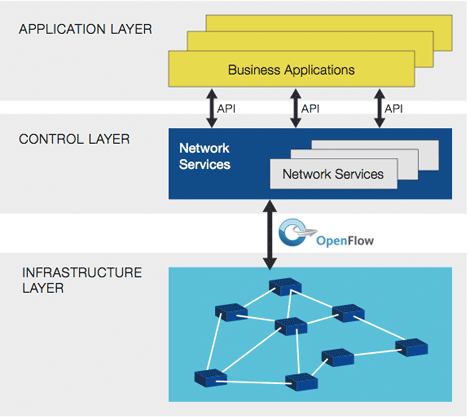
\includegraphics[scale=0.3]{SdnArchitecture.png}
\caption{\footnotesize SDN Architecture}
\end{figure}
\end{frame}






\begin{frame}
\section[]{Problem Statement}
\frametitle{Problem Statement}
\begin{itemize}
\footnotesize
\item
To develop a solution for the detection of DDoS attack in SDN environment using Support Vector Machine, Entropy Based Discretization, Fuzzy C Means Clustering and monitoring OpenFlow statistics.
\end{itemize}
\end{frame}




\begin{frame}
\section[]{Motivation}
\frametitle{Motivation}
\begin{center}
\begin{itemize}
\footnotesize
\item 
Number of cyber attacks is increasing day by day.
\item
Reluctance to adopt SDN due to lack of security solutions.
\item
A single DDoS attack can cost an enterprise over \$1.6 million.
\item
SDN market is expected to grow to \$56 Billion by 2022.
\item
Automation of attack detection is required.
\item
Integration of Machine Learning and Data Mining with SDN. 
\end{itemize}
\end{center}

\end{frame}



%\begin{frame}
% \frametitle{Literature Survey}
% \scriptsize
% \begin{center}
% \begin{tabular}{ | m{2cm} | m{2cm}| m{2cm} | m{3cm} | } 
% \hline
% \textbf{Title} & \textbf{Author} & \textbf{Journal and Year} & \textbf{Description} \\
% \hline
% DDoS Detection and Analysis in SDN-based Environment Using Support Vector Machine Classifier & 
% Kokila RT, S. Thamarai Selvi, Kannan Govindarajan & 
% IEEE 2014 & 
% This paper provides information about DDoS attack in SDN environment using Support Vector Machine to classify the attack.\\ 
% \hline
% An Entropy-Based Distributed DDoS Detection Mechanism in Software-Defined Networking &
% Rui Wang, Zhiping Jia, Lei Ju & 
% IEEE 2015 & 
% This paper provides information about DDoS attack in SDN environment using Entropy based mechanism to classify the attack.\\ 
% \hline
% Software-Defined Networking:The New Norm for Networks & 
% Open Networking Foundation & 
% ONF White Paper, 2012 & 
% Description about Software Defined Networks\\
% \hline
% Detection of DDoS Attacks using Enhanced Support Vector Machines with Real Time Generated Dataset & 
% T.Subbulakshmi, Dr. S. Mercy Shalinie, D. AnandK,  K.Kannatha&
% IEEE 2013 &
% Provided information how to create and use datasets for SVM.\\
% \hline
% OpenFlow Switch Specification& 
% Open Networking Foundation &
% Version 1.3.2 2013 &
% Description about OpenFlow Protocol\\
% \hline
% \end{tabular}
% \end{center}
% \end{frame}

\begin{frame}
\section[]{Objective}
\frametitle{Objective}
\begin{center}
\begin{itemize}
\footnotesize
%\item
%To compare different types of DDoS detection techniques.
\item
%To propose the best effective method for a specific environment.
To develop a system to detect DDoS attack in SDN.
\item
%To grasp an overview about the different network monitoring tools.
To monitor the network using Elasticsearch, Logstash and Kibana.
\item
To develop an adaptive solution for change in the  network.
\end{itemize}
\end{center}
\end{frame}

\begin{frame}
\section[]{Scope}
\frametitle{Scope}
\begin{center}
\begin{itemize}
\footnotesize
\item
%OpenFlow protocol in SDN switches.
Set up of SDN environment.
\item
SVM, Entropy and Fuzzy C Means based DDoS detection method.
\item
OpenFlow Monitoring application using POX API.
\end{itemize}
\end{center}
\end{frame}



%\begin{frame}
%\frametitle{Synopsis}
%\begin{center}
%\begin{itemize}
%\footnotesize
%\item
%SDN involves seperation of control and data plane.

%\item
%Security is a major concern in SDN architecture.

%\item
%DDoS attack results in exhaustion of controller resources.

%\item
%Entropy is a good measure of randomness.

%\item
%SVM is capable of decision making from uncertain information.

%\item
%Application for viewing OpenFlow statistics.
%\end{itemize}
%\end{center}
%\end{frame}


% \begin{frame}{
% \small
% \textbf{
% Scope
% }
% }
% \begin{itemize}
% \footnotesize
% \item
% Implementation of:
% \begin{itemize}
% \footnotesize
% \item
% Entropy mechanism.

% \item
% Support Vector Machine classifier.

% \item
% OpenFlow statistics monitoring application.
% \end{itemize}
% \end{itemize}
% \end{frame}

% \begin{frame}{
% \small
% \textbf{
% Architecture Diagram
% }
% }
% \begin{figure}[H]
% \includegraphics[scale=0.25]{Architecture_Diagram.png}
% \caption{
% System Architecture
% }
% \end{figure}
% \end{frame}


\begin{frame}
\section[]{Literature Survey}
\frametitle{Literature Survey}
\scriptsize
\begin{center}
\begin{tabular}{ | m{2cm} | m{2cm}| m{2cm} | m{3cm} | } 
\hline
\textbf{Title} & \textbf{Author} & \textbf{Journal and Year} & \textbf{Description} \\
\hline
DDoS Detection and Analysis in SDN-based Environment Using Support Vector Machine Classifier & 
Kokila RT, S. Thamarai Selvi, Kannan Govindarajan & 
IEEE 2014 & 
This paper provides information about DDoS attack in SDN environment using Support Vector Machine to classify the attack.\\ 
\hline
An Entropy-Based Distributed DDoS Detection Mechanism in Software-Defined Networking &
Rui Wang, Zhiping Jia, Lei Ju & 
IEEE 2015 & 
This paper provides information about DDoS attack in SDN environment using Entropy based mechanism to classify the attack.\\ 
\hline
Software-Defined Networking:The New Norm for Networks & 
Open Networking Foundation & 
ONF White Paper, 2012 & 
Description about Software Defined Networks\\
\hline
Advances in Fuzzy Clustering and its Applications & 
Jose Valente de Oliveira, Witold Pedrycz &
Wiley 2007 &
This book provides information about the algorithm for Fuzzy C Means Clustering.\\
\hline
OpenFlow Switch Specification& 
Open Networking Foundation &
Version 1.3.2 2013 &
Description about OpenFlow Protocol\\
\hline
\end{tabular}
\end{center}
\end{frame}



\begin{frame}
\section[]{Architecture Diagram}
\frametitle{Architecture Diagram}
\begin{figure}[H]
\includegraphics[scale=0.38]{myarch.png}
\caption{\footnotesize System Architecture}
\end{figure}
\end{frame}


\begin{frame}
\section[]{UML Diagrams}
\frametitle{UML Diagrams}
\begin{figure}
\includegraphics[scale=0.3]{use_case.png}
\caption{\footnotesize Use Case Diagram}
\end{figure}
\end{frame}

\begin{frame}
\frametitle{UML Diagrams}
\begin{figure}
\includegraphics[scale=0.35]{sequence.png}
\caption{\footnotesize Sequence Diagram}
\end{figure}
\end{frame}


\begin{frame}
\section[]{Mathematical Model}
\frametitle{Mathematical Model}
\footnotesize
$S = \lbrace \lbrace I \rbrace ,\lbrace P \rbrace ,\lbrace O \rbrace \rbrace $\newline\newline
$I = \lbrace N \rbrace$

\noindent
where,\\
$N = \lbrace $ Network Statistics $ \rbrace $, \\
$F =\lbrace F_{i} \mid F_{i} \in T , \forall i$ $ F_{i} =$ Individual entry $ \rbrace$, \\
$T = \lbrace $ Flow Table $ \rbrace$, \\
$F \subseteq N$
\newline

$P = \lbrace P_{EBD}, P_{SVM}, P_{FCM} \rbrace$
\newline

$O = \lbrace O_{EBD} \cup O_{SVM} \cup O_{FCM} \rbrace$

\end{frame}

\begin{frame}
\frametitle{Mathematical Model}
\footnotesize
$P_{EBD} $ $ (I_{EBD},$ $O_{EBD})$\\
$\lbrace$


\begin{itemize}
\footnotesize
\item $I_{EBD} = \lbrace U_{i} \mid U_{i} = ($ Dest. Addr., Count$),  $ $ U_{i}  \subset F_{i} \rbrace$

\item $P_{i} = \frac{C_{i}}{N}$  

\item $\varepsilon = \sum_{i=0}^{n} - P_{i} log P_{i}$

\item $\varepsilon_{n} = \frac{\varepsilon}{N} $

\item $(\lambda < \varepsilon_{n}) \rightarrow  $ $ (\beta = 0)$ \\ $(\lambda > \varepsilon_{n}) \rightarrow  $ $ (\beta = 1)$

\item $ O_{EBD} = \lbrace \beta \mid \beta \in (0, $ $1) \rbrace$
\end{itemize}
$ \rbrace$
\newline

$P_{SVM} $ $ (I_{SVM},$ $O_{SVM})$\\
$\lbrace$
\indent
\begin{itemize}
\footnotesize
\item $I_{SVM} = \lbrace V_{i} \mid V_{i} = ($ Src. Addr., Dest. Addr., Time, Prot.$) \rbrace$

\item $y = \overline{\omega} * x + b$ 

\item $(y \leq -1) \rightarrow  $ $ (\alpha = 1)$ \\ $(y \geq 1) \rightarrow  $ $ (\alpha = 0)$

\item $ O_{SVM} = \lbrace \alpha \mid \alpha \in (0, $ $1) \rbrace$
\end{itemize}
$ \rbrace$
\end{frame}

\begin{frame}
\frametitle{Mathematical Model}
\footnotesize
$P_{FCM} $ $ (I_{FCM},$ $O_{FCM})$\\
$\lbrace$
\indent
\begin{itemize}
\footnotesize
\item $I_{FCM} = \lbrace W_{i} \mid W_{i} = ($ Time, Dest. Addr., X $) \rbrace$

\item $P_{l}(z_{i}) = \sum_{j=1}^{X}  \epsilon ^ { - \alpha || z_{i} - z_{l} || ^{2}} $ 

\item $ u_{ij} = \frac{d_{ij}^{-\frac{2}{m-1}}}{\sum_{l=1}^{c} d_{lj}^{- \frac{2}{m-1}}} $

\item $ c_{ij} = \frac{\sum_{j=1}^{X} u_{ij}^{m}C_{j}}{\sum_{j=1}^{X} u_{ij}^{m}} $

\item $(y \leq u_{attack}) \rightarrow  $ $ (\gamma = 0)$ \\ $(y \geq u_{attack}) \rightarrow  $ $ (\gamma = 1)$

\item $ O_{FCM} = \lbrace \gamma \mid \gamma \in (0, $ $1) \rbrace$
\end{itemize}
$ \rbrace$

\end{frame}

\begin{frame}
%\section[]{Algorithmic Strategies}
\frametitle{Algorithmic Strategies : Entropy Based Discretization}
\begin{figure}
\includegraphics[scale=0.3]{EBD.png}
\caption{\footnotesize Flowchart: Entropy Based Discretization Mechanism}
\end{figure}
\end{frame}


\begin{frame}
%\section[]{Algorithmic Strategies}
\frametitle{Algorithmic Strategies : Fuzzy C-Means Clustering}
\begin{figure}
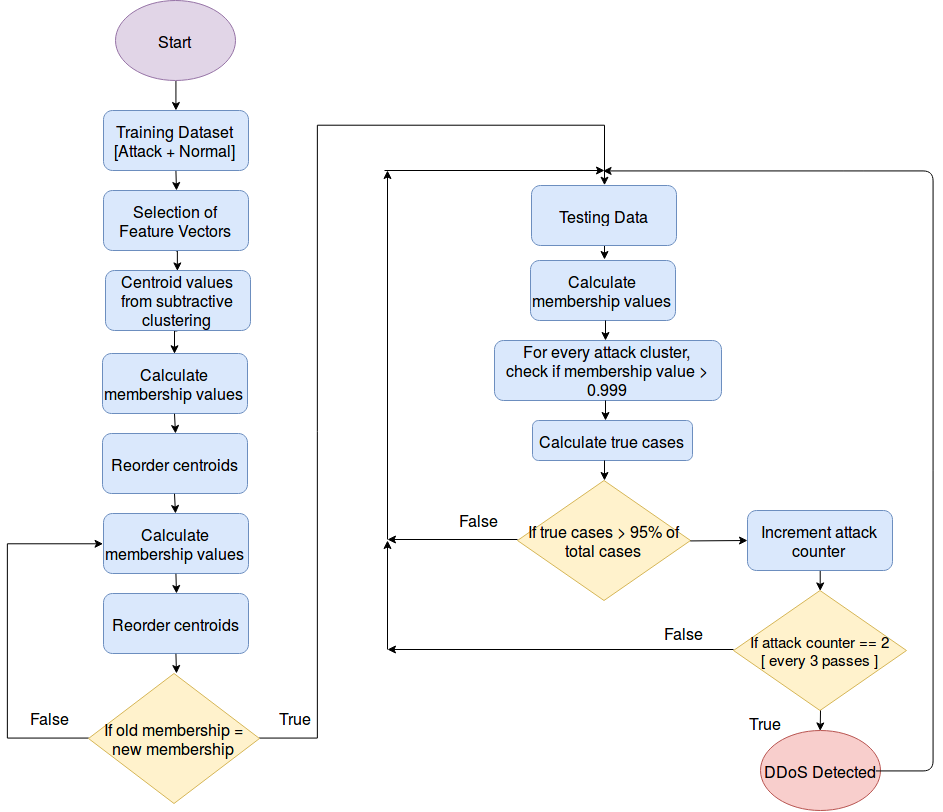
\includegraphics[scale=0.27]{fuzzy.png}
\caption{\footnotesize Flowchart: Fuzzy C Means Clustering}
\end{figure}
\end{frame}


\begin{frame}
\section[]{Algorithmic Strategies}
\frametitle{Algorithmic Strategies : Support Vector Machine}
\begin{figure}
\includegraphics[scale=0.3]{SVM.png}
\caption{\footnotesize Flowchart: Support Vector Machine Algorithm}
\end{figure}
\end{frame}



\begin{frame}
\frametitle{Algorithmic Strategies : Support Vector Machine}
\begin{figure}
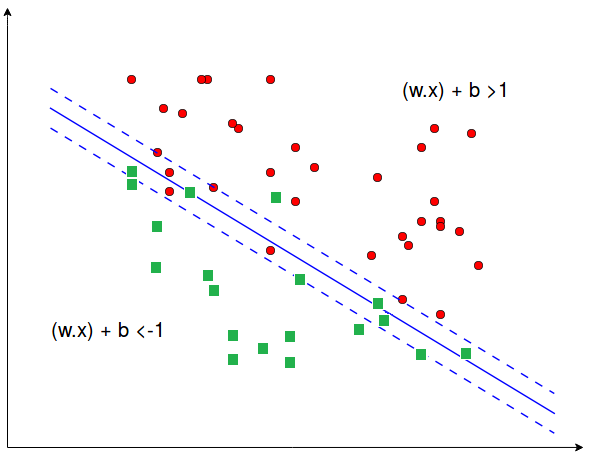
\includegraphics[scale=0.5]{Support_Vector_Machine.png}
\caption{\footnotesize Support Vector Machine Graph}
\end{figure}
\end{frame}

	

\begin{frame}
\section[]{Software Specifications}
\frametitle{Software Specifications}
\begin{itemize}
\footnotesize
\item
Linux based Operating System.
\item
Open vSwitch (OVS).
\item
Oracle VirtualBox.
\item
POX Controller.
\item
Python 2.7 or above.
\item
Mininet 2.2.1
\item
Flask
\item
Numpy, Pandas [Data analysis tools]
\item
tshark [CLI version of wireshark]
\item
Elasticsearch, Logstash, Kibana(ELK Stack)
\item
Watcher or ElastAlert
\item
sFlow-RT and hsflowd
\end{itemize}
\end{frame}

\begin{frame}
\section[]{Hardware Specifications}
\frametitle{Hardware Specifications}
\begin{itemize}
\footnotesize
\item
Any Enterprise/ Data Center/ Campus Network Topology with 1000+ Mbps.
\item
Manageable switches that support OpenFlow Protocol / Whitebox Switches.
\begin{itemize}
\footnotesize
\item
HPE Altoline 6900 48G ONIE AC Switch.
\item
Pica8 P-3297 48 X 1Gbe.
\item
HP 2920 Switch Series.
\end{itemize}

\item
Server Running the Controller
\begin{itemize}
\footnotesize
\item
Dell PowerEdge R720
\end{itemize}

\end{itemize}
\end{frame}



\begin{frame}
\section[]{Dataset Specifications}
\frametitle{Dataset Specifications}
\begin{itemize}
\footnotesize
\item
Dataset prepared using packet capturing tool tshark during both training and prediction phases.

\item
Training datasets include scenarios for both attack as well as normal nature of network.
\end{itemize}

\begin{table}
\scriptsize
\begin{center}
\begin{tabular}{ | m{1.5cm} | m{1.5cm}| m{1.5cm} | m{1cm} |} 
\hline
\textbf{Time Interval} & \textbf{Src. IP.} & \textbf{Dst. IP} & \textbf{Protocol} \\
\hline
0.025412000 & 192.168.1.11 & 192.168.1.13 & 1 \\
\hline
0.037555000 & 192.168.5.1 & 192.168.5.2 & 6 \\
\hline
0.024478000 & 192.168.1.11 & 192.168.1.13 & 1 \\
\hline
\end{tabular}
\end{center}
\caption{\footnotesize Normal Traffic Dataset}
\end{table}

\begin{table}
\scriptsize
\begin{center}
\begin{tabular}{ | m{1.5cm} | m{1.5cm}| m{1.5cm} | m{1cm} |} 
\hline
\textbf{Time Interval} & \textbf{Src. IP.} & \textbf{Dst. IP} & \textbf{Protocol} \\
\hline
0.000001000 & 192.168.1.14 & 192.168.1.11 & 1 \\
\hline
0.000002000 & 192.168.1.14 & 192.168.1.11 & 1 \\
\hline
0.000001000 & 192.168.1.14 & 192.168.1.11 & 1 \\
\hline
\end{tabular}
\end{center}
\caption{\footnotesize Attack Traffic Dataset}
\end{table}
\end{frame}


\begin{frame}
\section[]{Test Cases}
\frametitle{Test Cases}
\footnotesize
\begin{center}
\begin{tabular}{|p{0.5cm}|p{3.8cm}|p{2.2cm}|p{2.5cm}|}
\hline 
 \textbf{Id} & \textbf{Description} & \textbf{Scenario} & \textbf{Expected Output} \\ 
\hline 
 1 & Time span between attack detection and alert generation & Attack has occured & Instantaneous alert generation\\
 \hline
 2 & Normal Network Traffic, Log file not altered and attack is not detected & SDN functioning in normal mode & Alert not generated\\ 
\hline 
\end{tabular} 
\end{center}

\textbf{Scenario: Attack Traffic}
\begin{center}
\begin{tabular}{|p{0.5cm}|p{3.8cm}|p{2.2cm}|p{2.5cm}|}
\hline 
 \textbf{Id} & \textbf{Description} & \textbf{Input} & \textbf{Expected Output} \\ 
\hline 
 1 & Simple DoS attack & Large no. of same type of packets & Attack detected\\
 \hline
 2 & UDP flood attack & Large no. of UDP packets & Attack detected\\ 
 \hline
 3 & Varying DDoS attack bandwidth & Large no. of packets & DDoS attack should be detected only when bandwidth exceeds normal threshold traffic. \\
\hline 
\end{tabular} 
\end{center}
\end{frame}


\begin{frame}
\section[]{Results}
\frametitle{Results of Entropy Based Discretization}
\begin{itemize}
\footnotesize
\item
Switch configuration: Machine with Ubuntu 14.04, 8GB RAM, 4 logical cores
\item
Host configuration: Virtual Machine with Ubuntu 14.04, 1.5GB RAM, single core. 
\item 
POX controller.

\item
Normal traffic Rate: x pkts/second
\end{itemize}

\begin{table}
\scriptsize
\begin{center}
\begin{tabular}{ | m{2cm} | m{2cm}| m{2cm} | m{2cm} |} 
\hline
\textbf{Traffic Rate (pkts/second)} & \textbf{Entropy Values} \\
\hline
x &
0.854 \\
\hline
50x &
0.633 \\
\hline
%100x &
%0.517 \\
%\hline
200x &
0.511 \\
\hline
\end{tabular}
\end{center}
\caption{\footnotesize Entropy Values for different traffic rates}
\end{table}
\end{frame}




\begin{frame}
%\section[]{Results of Fuzzy C Means Clustering}
\frametitle{Results of Fuzzy C-Means Clustering}

\begin{itemize}
\footnotesize
\item
Normal and attack traffic datasets are generated at run time using tshark.

\item
Normal Traffic: x pkts/second
\newline
Normal Centroids: 0.00146, 2.1613

\item
Attack Traffic: 200x pkts/second
\newline
Attack Centroid: 0.000014
\end{itemize}

\begin{table}
\scriptsize
\begin{center}
\begin{tabular}{ | m{2cm} | m{2cm}| m{2cm} | m{2cm} |} 
\hline
\textbf{Traffic Rate(pkts/second)} & \textbf{\% attack packets in attack cluster} \\
\hline
x &
56\% \\
\hline
50x &
78\% \\
\hline
% 100x &
% 87\% \\
% \hline
200x &
99\% \\
\hline
\end{tabular}
\end{center}
\caption{\footnotesize Accuracy with different parameters}
\end{table}
\end{frame}

\begin{frame}
%\section[]{Results of SVM based Method}
\frametitle{Results of SVM based Method}

\begin{itemize}
\footnotesize

\item
Normal and attack traffic datasets are generated at run time using tshark.

\item
Attack to Total Ratio: Total attack classifications / Total number of packets
\end{itemize}

\begin{table}
\scriptsize
\begin{center}
\begin{tabular}{ | m{2cm} | m{2cm}| m{2cm} | m{2cm} |} 
\hline
\textbf{Traffic Rate (pkts/second)} & \textbf{SVM percentage Values} \\
\hline
x &
71\% \\
\hline
50x &
80\% \\
\hline
% 100x &
% 0.00002 \\
% \hline
200x &
99\% \\
\hline
\end{tabular}
\end{center}
\caption{\footnotesize SVM Ratio Values for different traffic rates}
\end{table}
\end{frame}


\begin{frame}
\frametitle{Performance Analysis}
%\section[]{Performance Analysis}
\footnotesize

\begin{figure}
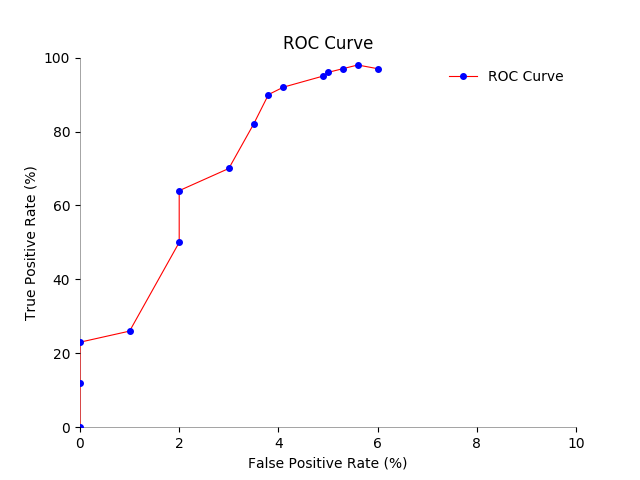
\includegraphics[scale=0.251]{2.png}
\caption{Reciever Operating Characteristic Curve}
\end{figure}

The performance analysis factors for the system are:
\begin{itemize}

\item
Accuracy: 95.33\%

\item
Detection Rate: 97.43\%

\item
False Positive Rate: 6.9\%
\end{itemize}
\end{frame}


\begin{frame}
\section[]{Conclusion}
\frametitle{Conclusion}

\footnotesize
\begin{itemize}
\item
%Proposing a solution for DDoS detection in SDN environment and also comparing the effectiveness of both methods (SVM, Entropy based Discretization and Fuzzy C Means Clustering) in a specific environment which would be a step towards solving the security issues and accelerating the adoption of SDN.

Hence, we build a solution which can be used for detecting flooding type of DDoS attacks. For this purpose we use three algorithms operating during runtime that utilize less resources with high accuracy and high detection rate. Thus taking a step towards solving the security issues and accelerating the adoption of SDN.

\end{itemize}
\end{frame}


\begin{frame}
\section[]{References}
\frametitle{References}
\begin{itemize}
\footnotesize
\item
"DDoS Detection and Analysis in SDN-based Environment Using Support Vector Machine Classifier" - Kokila RT, S. Thamarai Selvi, Kannan Govindarajan - 2014 Sixth International Conference on Advanced Computing(ICoAC) - Department of Computer Technology, Anna University (MIT Campus), Chennai.

\item
"An Entropy-Based Distributed DDoS Detection Mechanism in Software-Defined Networking" - Rui Wang, Zhiping Jia, Lei Ju - 2015 IEEE Trustcom/BigDataSE/ISPA - School of Computer Science and Technology Shandong University Jinan, China.

\item
"Software-Defined Networking:The New Norm for Networks and 
Open Networking Foundation" - Open Networking Foundation - ONF White Paper April 13, 2012.

\item
"Advances in Fuzzy Clustering and its Applications" -
Jose Valente de Oliveira, Witold Pedrycz
Wiley 2007

\item
T.Subbulakshmi , Dr. S. Mercy Shalinie, V.GanapathiSubramanian, K.BalaKrishnan, D. AnandK, K.Kannathal - IEEE-ICoAC 2011 - Department of CSE, TCE Madurai, India.

\item
"OpenFlow Switch Specification" - Open Networking Foundation - Version 1.3.2 2013.

\end{itemize}
\end{frame}

\begin{frame}{}
\Huge
\centering
\textbf{Thank You\ldots}
\end{frame}

\begin{frame}{}
\Huge
\centering
\textbf{Demo}
\end{frame}


\end{document}